\documentclass[11pt,a4paper]{article}

\usepackage{kotex}
\usepackage{datetime}
\usepackage{framed}
\usepackage{fullpage}
\usepackage{graphicx}
\usepackage{float}
\usepackage[english]{babel}
\graphicspath{ {images/} }

\newdateformat{koreandate}{\THEYEAR년 \twodigit{\THEMONTH}월 \twodigit{\THEDAY}일}

\begin{document}
\title{예약한 강의실의 접근성 및 이용 편의성 개선 방안}
\author{
김슬기\\
김재찬\\
김찬민\\
심규민\\
유재성
}
\date{}
\maketitle

\begin{framed}

\centerline{\textless배움의 윤리 서약\textgreater}

\begin{enumerate}
\item 이 과제물은 내가(우리가) 직접 연구하여 작성한 것이다.
\item 정확한 출처 제시 없이 다른 사람의 글이나 생각을 가져오지 않았다.
\item 인용한 문헌의 내용이나 자료(도표나 데이터)를 조작(위조 혹은 변조)하지 않았다.
\item 과제물을 다른 사람으로부터 받거나 구매하여 제출하지 않았다.
\item 과제물 작성에 참여하지 않은 사람을 공동 제출자로 명기하지 않았다.
\end{enumerate}

\begin{center}
이 과제물은 위의 항목들을 준수하여 작성한 것임을 확인합니다.\\
\hfill\break
\koreandate\today\\
\hfill\break
작성자\\
\hfill\break
김슬기 (서명)\\
김재찬 (서명)\\
김찬민 (서명)\\
심규민 (서명)\\
유재성 (서명)
\end{center}

\end{framed}

\thispagestyle{empty}
\pagebreak
\pagenumbering{roman}
\setcounter{page}{1}
\renewcommand{\abstractname}{초록}
\begin{abstract}
본 논문에서는 서울대학교 강의실 예약 시스템을 통해 예약한 강의실의 접근성과 그
강의실을 이용할 때까지 발생할 수 있는 불편함을 해소하여 편의성을 개선할 방안을
제시한다. 기존의 시스템은 제삼자인 수위의 도움을 받아야 문을 열 수 있는 등
강의실 접근성이 떨어지며, 인증을 해주는 수위가 자리를 비울 경우 강의실을
이용하지 못할 수도 있다. 본 연구에서는 우선 설문조사를 통해 이러한 문제가
실제로 존재하는지 보였다. 예약한 강의실 문이 잠겨 있는 것을 경험한 사용자는
전체의 절반이나 되었다. 문제를 해결할 수 있는 방안으로 블랙 리스트 모델과
화이트 리스트 모델을 제시하였다. 제시한 모델이 문제를 잘 해결할 수 있는지
검증하기 위해, 기존 모델과 제시한 모델들을 형식화하고 이를 프롤로그 언어로
프로그램을 작성하여 비교하였다. 그 결과 약한 블랙 리스트 모델은 오히려 기존
모델보다 불편하였고, 강한 블랙 리스트 모델과 화이트 리스트 모델은 모두 기존
모델의 기능을 잘 수행하면서, 불편한 점을 개선할 수 있었다.\\
\centerline{핵심어: 강의실, 수위, 예약, 잠금장치, 일회성 비밀번호, 이미지 프로세싱}
\end{abstract}
\pagebreak

\renewcommand{\contentsname}{목차}
\tableofcontents

\pagebreak
\pagenumbering{arabic}
\setcounter{page}{1}
\section{서론}

\subsection{연구 목적}
서울대학교 학생들은 수업시간 외에 강의실을 이용하려면 강의실 예약 시스템을 통해
강의실을 예약하고 이용해야 한다. 그런데 예약한 시간에 강의실에 도착하여도
강의실 문이 잠겨 있어서 수위의 도움을 받아야 문을 열 수 있는 등 강의실 접근에
불편함이 있고, 그에 따르는 몇 가지 문제점이 생긴다. 수위가 인터넷을 사용할 수
있다면 예약 신청을 확인할 수 있지만, 그렇지 않으면 예약자가 신청서를 따로
제출해야 하는 번거로움이 있다. 또 인증을 해주는 수위가 자리를 비울 경우
강의실을 이용하지 못할 수도 있다. 이 연구는 서울대학교 강의실 예약 시스템을
통해 예약한 강의실을 예약자가 실제로 이용할 때까지 겪을 수 있는 불편의 해소를
목적으로 한다.

\subsection{연구 범위}
강의실 예약하는 과정은 예약 시스템이 담당하고 있는 부분으로서, 이 연구에서
다루지 않는다. 이 연구에서는 문제 해결을 위해 두 가지 모델을 제시하고, 두
모델이 문제 상황을 얼마나 잘 해결할 수 있는지 검증한다. 즉, 기존의 강의실 이용
방법이 삼자 인증을 통한 시스템이었다면, 이 연구에서는 블랙 리스트 모델과 화이트
리스트 모델을 이용한 시스템을 제안한다.

\section{선행연구}

\subsection{용어정의}
블랙 리스트(Black List) 모델이란, 평소에는 강의실에 접근하는 것을 차단하지 않고
특정 대상, 즉 예약되어 있지 않은 강의실을 이용하는 사람들을 걸러내어 사용을
금지하는 모델을 말한다.

화이트 리스트(White List) 모델이란, 기본적으로는 강의실 접근을 차단하되, 접근이
허가된 사람들만 들여보내는 모델이다. 일반적으로 많이 쓰이는 모델로, 가장 흔히
볼 수 있는 모델은 열쇠와 자물쇠이다.

삼자 인증을 통한 시스템이란, 정당한 인증을 받은 사용자라도 이를 확인하기 위해
제삼자(이 연구에선 예약한 사용자인지 확인하고 문을 열어주는 수위)의 추가적인
인증을 통해 접근 권한을 따로 얻는 방식이며, 현행 강의실 예약 시스템이 이에
해당한다.

예약자란, 강의실 예약을 실제로 행한 사람을 말한다. 예약자는 특정 시간에 한해
예약한 강의실에 대한 정당한 사용 권한을 가지고 있다.

허가된 사용자란, 예약자와 함께 특정 시간에 한해 예약한 강의실을 이용할 수 있는
사람으로서, 예약자 또한 허가된 사용자에 포함된다. 일반적으로 강의실은 두 명
이상이 이용할 목적으로 예약하기 때문에, 허가된 사용자는 두 명 이상이다.

불허된 사용자란, 특정 시간과 강의실에 대해 그 강의실을 이용하는 것이 허가되지
않은 사람이다. 예약 없이 몰래 비어 있는 강의실을 이용하려고 하는 경우나, 허가된
사용자가 아님에도 사용 중인 강의실에 들어가는 경우가 이에 해당한다.

\subsection{이론적 배경}

\subsubsection{일회용 비밀번호(OTP) 잠금장치(Door Lock) 특허}
이 발명은 난수를 이용한 전자식 잠금장치 및 그 제어방법에 관한 것으로서, 좀 더
세부적으로 말하자면 일정한 자릿수를 갖는 난수를 발생시킨 뒤에 위치지정번호에
해당하는 번호를 추출하고, 이를 반복횟수번호에 따라 일정 횟수 반복하면서 최종
위치지정번호에 해당하는 번호를 추출하여 비밀번호로 사용함으로써 비밀번호의
유출을 방지할 수 있는, 난수를 이용한 전자식 잠금장치 및 그 제어방법에 관한
것이다.

\subsubsection{영상 처리}
영상 처리(Image Processing)는 사진이나 동영상을 입력으로 하여 정보를 처리하는
기술이다. 영상 처리를 이용하면 폐쇄 회로와 같은 카메라가 촬영한 영상을 실시간
또는 정적으로 분석하여, 움직임 인식(Motion Detection), 글자 인식(OCR) 등을 할
수 있다. 이를 응용하면 물건이나 사람을 구분할 수 있다. 이 기술은 보안 목적이나
자동차 번호판 인식 등에 활용되고 있다.

\subsubsection{컴퓨터를 이용한 추론}
프롤로그(Prolog)는 일차 술어 논리(First Order Logic)를 사용하는 프로그래밍
언어이다. 언어의 구성 요소는 크게 사실(Fact), 규칙(Rule)과 질의(Query)가 있다.
사실은 어떠한 것이 사실이라고 선언하는 요소이다. 규칙은 ‘ㄱ이면 ㄴ이다’를
서술해주는 요소이다. 질의는 주어진 논리식이 사실인지 아닌지 물어보는 요소이다.
프롤로그 프로그램이 수행되면, 질의가 주어진 조건을 만족하는 것이 있는지
추론해낸다. 만약 만족하는 것이 있다면 주어진 논리식의 자유 변수(Free
Variable)가 어떤 경우에 참인지 알려준다. 만약 만족하는 것이 없다면 그렇다는
결과를 돌려준다.

프롤로그를 이용한 증명 시스템도 개발되어 있다. 그중 하나인 프롤로그 기술 정리
증명기(Prolog Technology Theorem Prover)라고 이름 지어진 소프트웨어는 정리를
증명하는 데 사용될 수 있다.

\section{연구 방법과 절차}
논문의 주제인 예약한 강의실 사용 문제를 정확하게 파악하기 위해 설문조사를
만들었다. 설문조사의 답변을 통해 문제를 확인하고, 예약한 강의실의 접근성 및
이용 편의성 개선을 위해 몇 가지 모델을 제시한다. 마지막으로, 제시된 모델들이
설문조사의 답변을 통해 확인된 문제들을 실제로 해결하는지 컴퓨터 프로그래밍을
이용한 자동화 검증 시스템으로 확인한다.

\subsection{문제의 발견 : 설문조사}

\subsubsection{설문조사의 필요성}
논문의 주제인 예약한 강의실 사용 문제를 구체화하기 위해 몇 가지 항목에 대해 설문조사 할 필요가 있다.
첫 번째, 이용자들이 예약한 강의실을 실제로 사용할 때 어떤 불편 함들을 겪는지 조사해야 한다.
그리고 어떤 문제들의 해결에 집중해야 하는지 파악하기 위해 이용자들이 이 불편 함들을 얼마나 느끼는지 그 비율을 조사해야 한다.
마지막으로 불편함으로는 간과될 수 있는 문제들을 파악하기 위해 예약한 강의실을 사용할 때 생길 수 있는 특정 문제에 대한 이용자들의 인식을 조사할 필요가 있다.

\subsubsection{설문조사의 내용}
문제의 구체화에 필요한 질문들로 설문조사를 구성한다. 우선 서울대학교 학생들이 강의실 예약 시스템을 얼마나 이용하는지 파악한다. 그리고 강의실 예약 시스템을 이용해서 주로 예약하는 강의실 분포를 확인하기 위해 설문하는 학생들의 소속 단과대학을 조사한다.
강의실 예약 시스템을 통해 예약한 강의실을 실제로 사용할 때 겪는 문제들을 정확히 파악하고 그 비율을 알아보기 위해 강의실 예약 시스템을 이용해본 학생들을 대상으로 예상되는 여러 불편한 점 중에서 실제 경험해본 불편한 점들을 선택하도록 한다.
마지막으로 문제들을 해결할 때 어떤 문제에 집중해서 해결해야 하는지를 파악하기 위해서 예약한 강의실을 사용할 때 생긴다고 예상되는 특정 문제들에 대한 중요성을 점수형태로 설문한다.

\subsubsection{설문조사의 설문 범위}
현재 강의실 예약 시스템으로 강의실 예약 신청이 가능한 단과대학은 인문대학, 사범대학, 약학대학, 공과대학, 농업생명과학대학, 자연과학대학, 사회과학대학, 미술대학이다.
강의실 예약 시스템이 대부분 단과대학의 강의실 예약을 포함하고 있기 때문에 학교 전체를 대상으로 설문조사를 진행한다.

\subsection{문제의 해결}
우리는 강의실 사용의 문제를 해결하기 위해서 두 가지 모델을 도입할 것이다.
하나는 블랙 리스트라고 불리는 것으로 특정 대상만을 걸러내어 사용을 금지하는
방식이고, 다른 하나는 화이트 리스트라고 불리는 것으로 허가된 사용자만 강의실을
사용할 수 있게 하는 방식이다.

\subsubsection{블랙 리스트 모델}
위에서 언급한 대로 일반적으로 접근을 허용하고, 특정 대상만을 걸러내어 사용을
금지하는 방식을 블랙 리스트 방식이라고 한다. 우리는 이 모델을 강의실에 적용하기
위하여 CCTV와 이미지 프로세싱 기술을 이용할 것이다. 이미 예약 시스템은
인터넷으로 구현되어 있기 때문에 예약 시간은 전부 전산화되어 관리되고 있고,
보안상의 이유로 많은 강의실에는 CCTV가 설치되어 있다. 우리가 제시하는 블랙
리스트 모델은 이 정보들을 적극적으로 이용하여 Visual surveillance라고 불리는
감시 기법을 사용할 것이다.

블랙 리스트 모델이 기존의 시스템과 다른 가장 큰 차이점은 모든 강의실을 개방해
둘 수 있다는 것이다. 우리는 이미 전산화된 예약 정보를 가지고 있다. 이 정보를
바탕으로 현재 강의실에 사람이 있을 때 그 사람이 사용이 허락된 사람인지 아닌지를
추정할 수 있다.

\subsubsection{화이트 리스트 모델}
화이트 리스트 모델은 블랙 리스트 모델과 다르게 기본적으로 문은 잠겨 있고 허락된
사람만 사용할 수 있게 하는 모델이다. 사실 기존 시스템도 화이트 리스트
모델이라고 할 수 있다. 다만, 기존 시스템은 허락된 사람인지를 수위를 통해서
확인할 수 있다는 것에서 불편함이 있었다. 고전적인 자물쇠에서는 이 문제를 해결할
수 없다. 그래서 새로 도입할 시스템에서는 새로운 인증 시스템을 도입해야 한다.

새로 도입할 인증 시스템의 필요조건은 다음과 같아야 한다. 우선, 예약자가 키에
접근하는데 제삼자에게 인증받아서는 안 된다. 이런 시스템은 결국 수위가
인증해주던 기존의 시스템과 다를 바 없다. 또 다른 요구사항은 예약자 본인이
아니더라도 예약자의 일행이라도 잠겨 있는 문을 열 수 있어야 한다는 것이다.
따라서 공유할 수 없는 물리적인 키를 이용한 시스템, 혹은 사용에 예약자의 개인
정보가 있어야 하는 방식은 사용할 수 없다. 마지막 요구사항으로 예약한 시간이
아니면 강의실을 이용할 수 없어야 한다는 것을 생각할 수 있다. 즉, 한번 키를 받고
그 뒤로 키를 반납하지 않고 사용할 수 있는 시스템은 사용해서는 안 된다는 것이다.
이런 문제로 기존의 디지털 자물쇠는 사용할 수 없다.

우리는 위에서 말한 조건들을 만족하는 OTP(One-Time Password)를 이용할 것이다.
OTP는 시간 정보를 기반으로 한정된 시간 내에만 사용 가능한 비밀번호를 생성하는
방식으로 은행 등에서 많이 사용되는 기술이다.

특정 시간대에 사용하기 위해서 만들어진 암호는 해당 시간대에서만 사용 가능하므로
유출되었을 때의 위험도 없고, 물리적인 키가 아니므로 예약자가 일행들에게
공유하기도 쉽다.

\subsection{문제 해결책 검증}

\subsubsection{모델의 형식화}
강의실을 예약하고 이용할 때 마땅히 만족해야 할 성질들이 있다. 예를 들면,
강의실을 예약한 사람은 예약한 시간에 해당 강의실을 이용할 수 있어야 한다.
이러한 성질들을 모아 일차 술어 논리의 형태로 기술해볼 수 있다. 나아가 각 모델을
적용하였을 때 해결되길 기대하는 성질들도 있다. 이것들도 마찬가지 형태로 표현할
수 있다.

\subsubsection{성질의 증명}
각 모델이 만족해야 할(또는 만족하길 기대하는) 성질들에 대해, 모델별로 그
성질들을 얼마나 만족하는지, 만족하지 못한다면 어떤 경우에 만족하지 않는지
확인할 것이다. 각 성질의 상황을 서술하는 명제와 모델의 규칙 나타내는 명제를
이용하여 확인할 것이다.

각 모델을 일차 술어 논리로 형식화하면, 앞서 소개한 프롤로그를 통해 이러한
확인을 할 수 있다. 검증에 필요한 명제들을 프롤로그 언어로 작성하여 프로그램을
만들 수 있다. 이 프로그램을 프롤로그의 구현체인 SWI-Prolog(버전 6.6.6)를
사용하여 실행할 것이다.

\section{연구 결과}

\subsection{문제의 발견 : 설문조사 결과}

\subsubsection{설문조사 응답 분석}
온라인으로 진행한 설문조사의 응답 수는 54명으로 다양한 단과대 표본을 얻지 못해
오프라인 설문조사를 진행했다. 오프라인 설문조사 응답 수는 248명이다. 따라서
설문조사 총 응답 수는 302명이다. 첫 번째 문항으로 설문한 강의실 예약 시스템
이용 경험에서는 경험이 있는 설문조사 응답 수는 84명이고 경험이 없는 설문조사
응답 수는 218명이다. 따라서 84 / 218 = 38.5\%의 강의실 예약 시스템 이용
경험률을 확인할 수 있다.

충분한 설문조사 응답 수를 확보하지 못한 단과대학들이 있다. 해당 단과대학들은
다른 단과대학들에 비해 상대적으로 학생 수가 적고 지정된 강의동에서만 수업이
이뤄지는 단과대학들이다. 간호대학의 응답 수는 1명, 법대, 수의대, 약대,
음/미대의 응답 수는 0명이다. 응답 수가 거의 없으므로 설문조사 결과해석에서
고려되지 않는다.

어느 정도의 설문조사 응답 수를 확보한 단과대학 중에서 강의실 예약 시스템
이용률이 현저하게 떨어지는 단과대학들을 확인할 수 있다. 상대적으로 해당
단과대학의 수업들이 수업의 과제 중에 조별 과제가 적다고 추측할 수 있지만,
강의실 예약 시스템을 이용하지 않는 이유에 대해서는 설문조사 하지 않았기 때문에
명확한 이유는 파악하기 어려우며 추가적인 조사가 필요하다. 생활과학대의 응답
수는 10명 중 강의실 예약 시스템 이용 경험 수는 1명, 의대는 7명 중 1명, 자연대는
24명 중 1명 마지막으로 자유전공은 12명 중 1명이다. 전체 설문조사 결과에서는
강의실 예약 시스템 이용 경험률이 38.5\% 정도로 높으므로 이 단과대학에서는
설문조사 결과해석이 정확히 적용되지 않을 수 있다.

\subsubsection{여러 불편한 점 경험률 분석}
강의실 예약 시스템을 이용해본 학생들을 대상으로 예상되는 여러 불편한 점 중에서
실제 경험해본 불편한 점들을 조사했다. 가장 많은 응답자가 불편을 겪었다고 답한
문항은 6번과 7번 문항이다. 6번 문항은 강의실 이용 중에 강의실 예약 시간 연장의
필요성을 느꼈다는 것이고 7번 문항은 이미 예약한 시간을 변경하거나 취소해야 하는
문제가 있다는 문항이다. 이 두 문항은 강의실 예약 시스템 이용 경험이 있는 응답
수의 51\%에 해당한다. 따라서 많은 이용자가 강의실을 예약한 시간과 실제 강의실을
이용하는 시간이 다른 경험이 많다는 것을 알 수 있다. 또, 강의실 예약 시스템에서
예약 시간을 변경했을 때 실제 강의실 이용에 불편함이 없어야 한다는 것도 알 수
있다.

다음으로 가장 많은 응답자가 불편함을 느꼈다고 답한 문항은 4번과 3번이다. 4번
문항은 강의실 예약 시스템을 통해 강의실을 예약한 다음 예약한 강의실에 갔을 때
문이 잠겨있었다는 문항이고, 3번 문항은 같은 4번과 같은 상황에서 수위가 자리를
비운 상태였다는 문항이다. 두 문항은 강의실 예약 시스템 이용 경험이 있는 응답의
50\%, 36.9\%에 해당했다. 따라서 많은 이용자가 예약한 강의실에 갔을 때 강의실이
잠겨있어 강의실을 바로 사용하지 못했다는 것을 알 수 있다. 또, 잠겨있는 강의실을
열기 위해 수위를 찾았을 때 높은 확률로(36.9 / 50 = 73.8\%) 수위가 자리를
비웠다는 것도 알 수 있다.

위 분석에 따르면 높은 경험률을 보였던 예약 시간문제와 강의실 출입 문제가 가장 큰 문제점들이라는 것을 알 수 있다.
\begin{figure}[h]
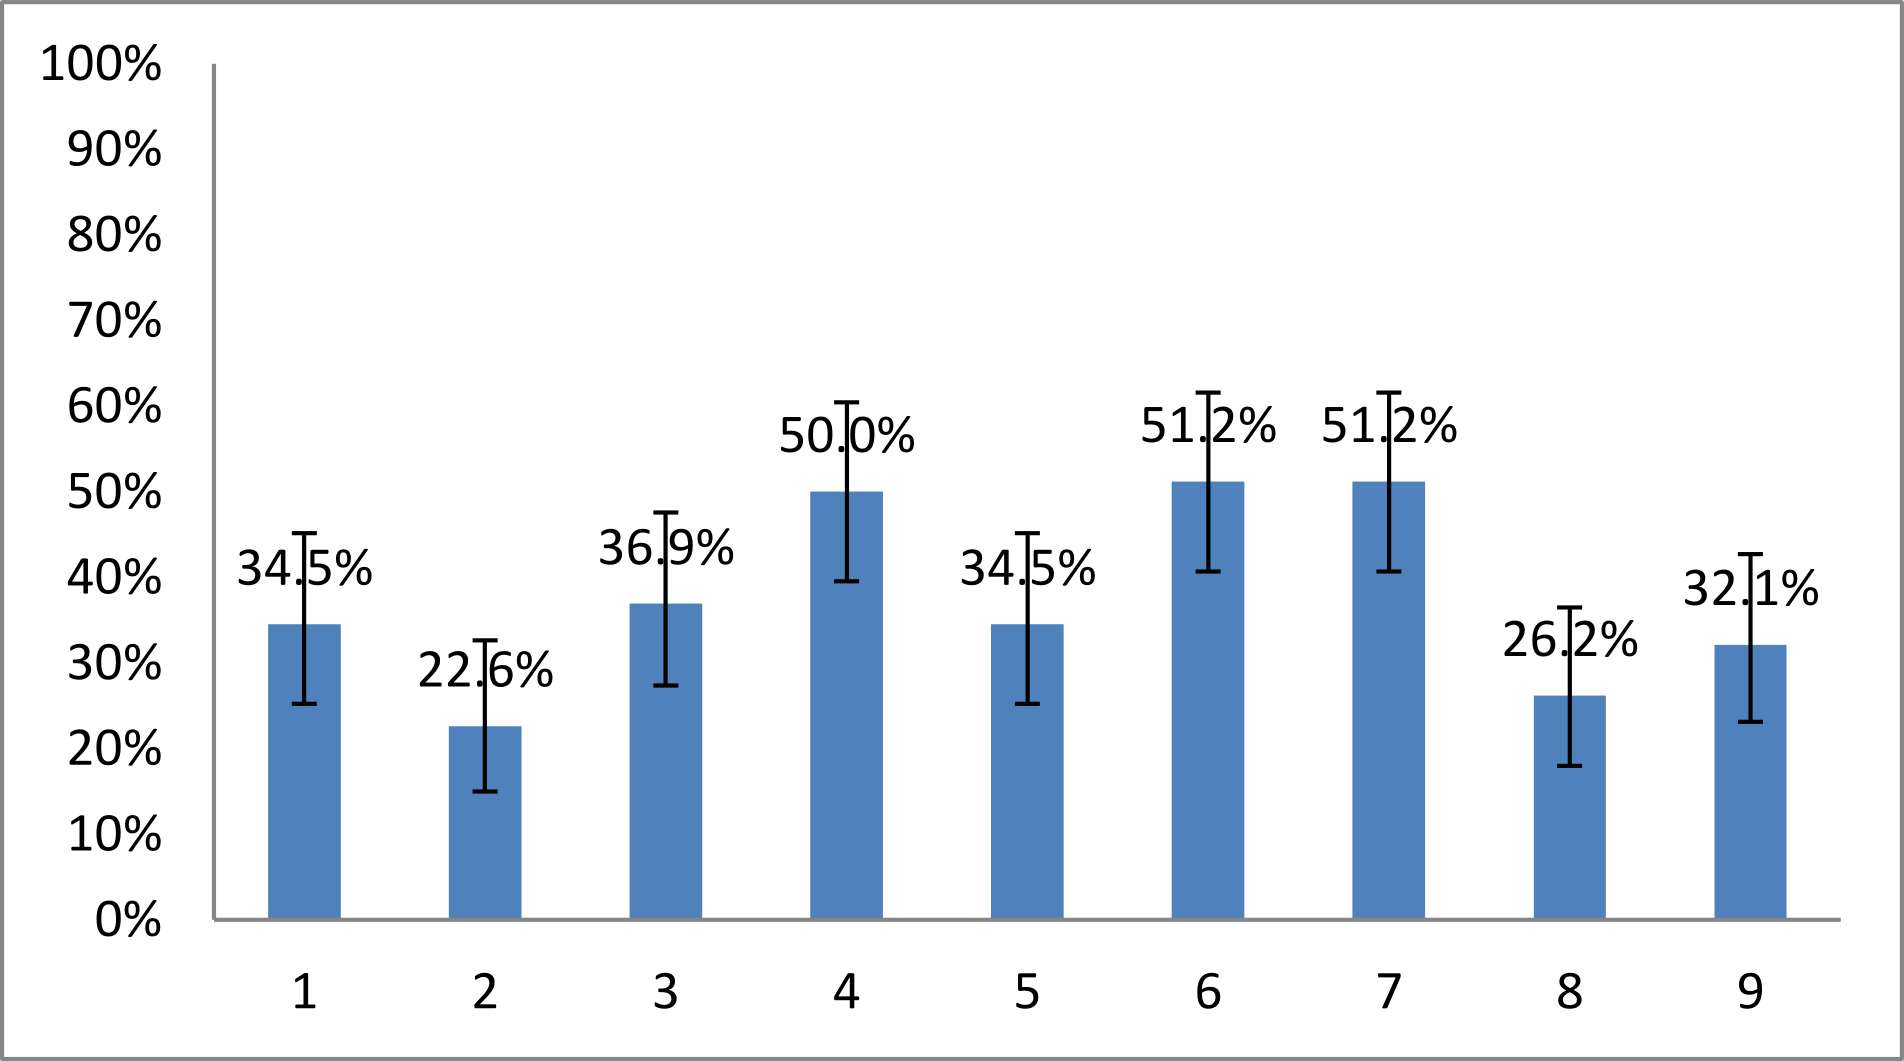
\includegraphics[width=0.8\textwidth]{4_1_2}
\centering
\end{figure}

\subsubsection{여러 불편한 점 경험률 단과대학별 분석}
강의실 예약 시스템을 이용해보았다는 응답 수가 가장 많았던 윗공대는 설문조사
전체의 응답률이 유사하다는 것을 알 수 있다. 표본 수가 많을수록 전체 결과에 많은
영향을 주기 때문이라고 해석할 수 있다. 응답 수 대비 강의실 예약 시스템 이용
경험률이 가장 높은 사범대의 결과는 설문조사 전체의 응답률과 대부분 유사한
결과를 보여주지만 1번 항목인 강의실 예약 후 예약했는지를 확인하기 위해 수위에게
예약 신청서를 요구받은 적이 있다는 응답률은 특히 높았고(66.6\%), 5번 항목인
예약하지 않은 사람들이 예약한 강의실을 선점해서 사용하고 있었다는 경험의
응답률은 특히 낮았다. (22.2\%) 이것은 사범대 수위가 강의실 예약 시스템에서
발급하는 예약 확인서 확인을 철저하게 했고, 따라서 예약하지 않은 사용자들이
강의실을 선점해서 사용하는 경우가 적었다고 해석할 수 있다.

반면에 충분한 수의 응답을 확보하지 못한 단과대학과 예약 시스템 예약률이
현저하게 떨어지는 단과대학을 제외한 단과대학 중 예약 경험 표본이 가장 적은
인문대와 예약 경험률이 가장 낮은 사회대는 전체 결과와는 다르다는 것을 알 수
있다. 이것은 강의실 예약 시스템 경험이 많을수록 강의실 이용의 불편함을 겪을
확률이 높다는 것을 방증한다. 그럼에도 불구하고 가장 큰 문제점들로 지적되었던
항목들에서는 여느 정도의 응답률이 있다는 것 또한 확인할 수 있다. 인문대의 3, 4,
6, 7항목은 0\%, 33.3\%, 66.6\%, 33.3\%, 사회대는 0\%, 25\%, 50\%, 25\%의
응답률을 보였다.
\begin{figure}[h]
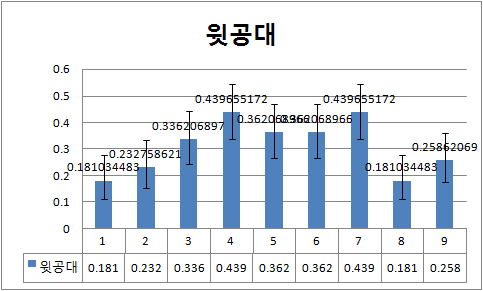
\includegraphics[width=0.45\textwidth]{4_1_3_1}
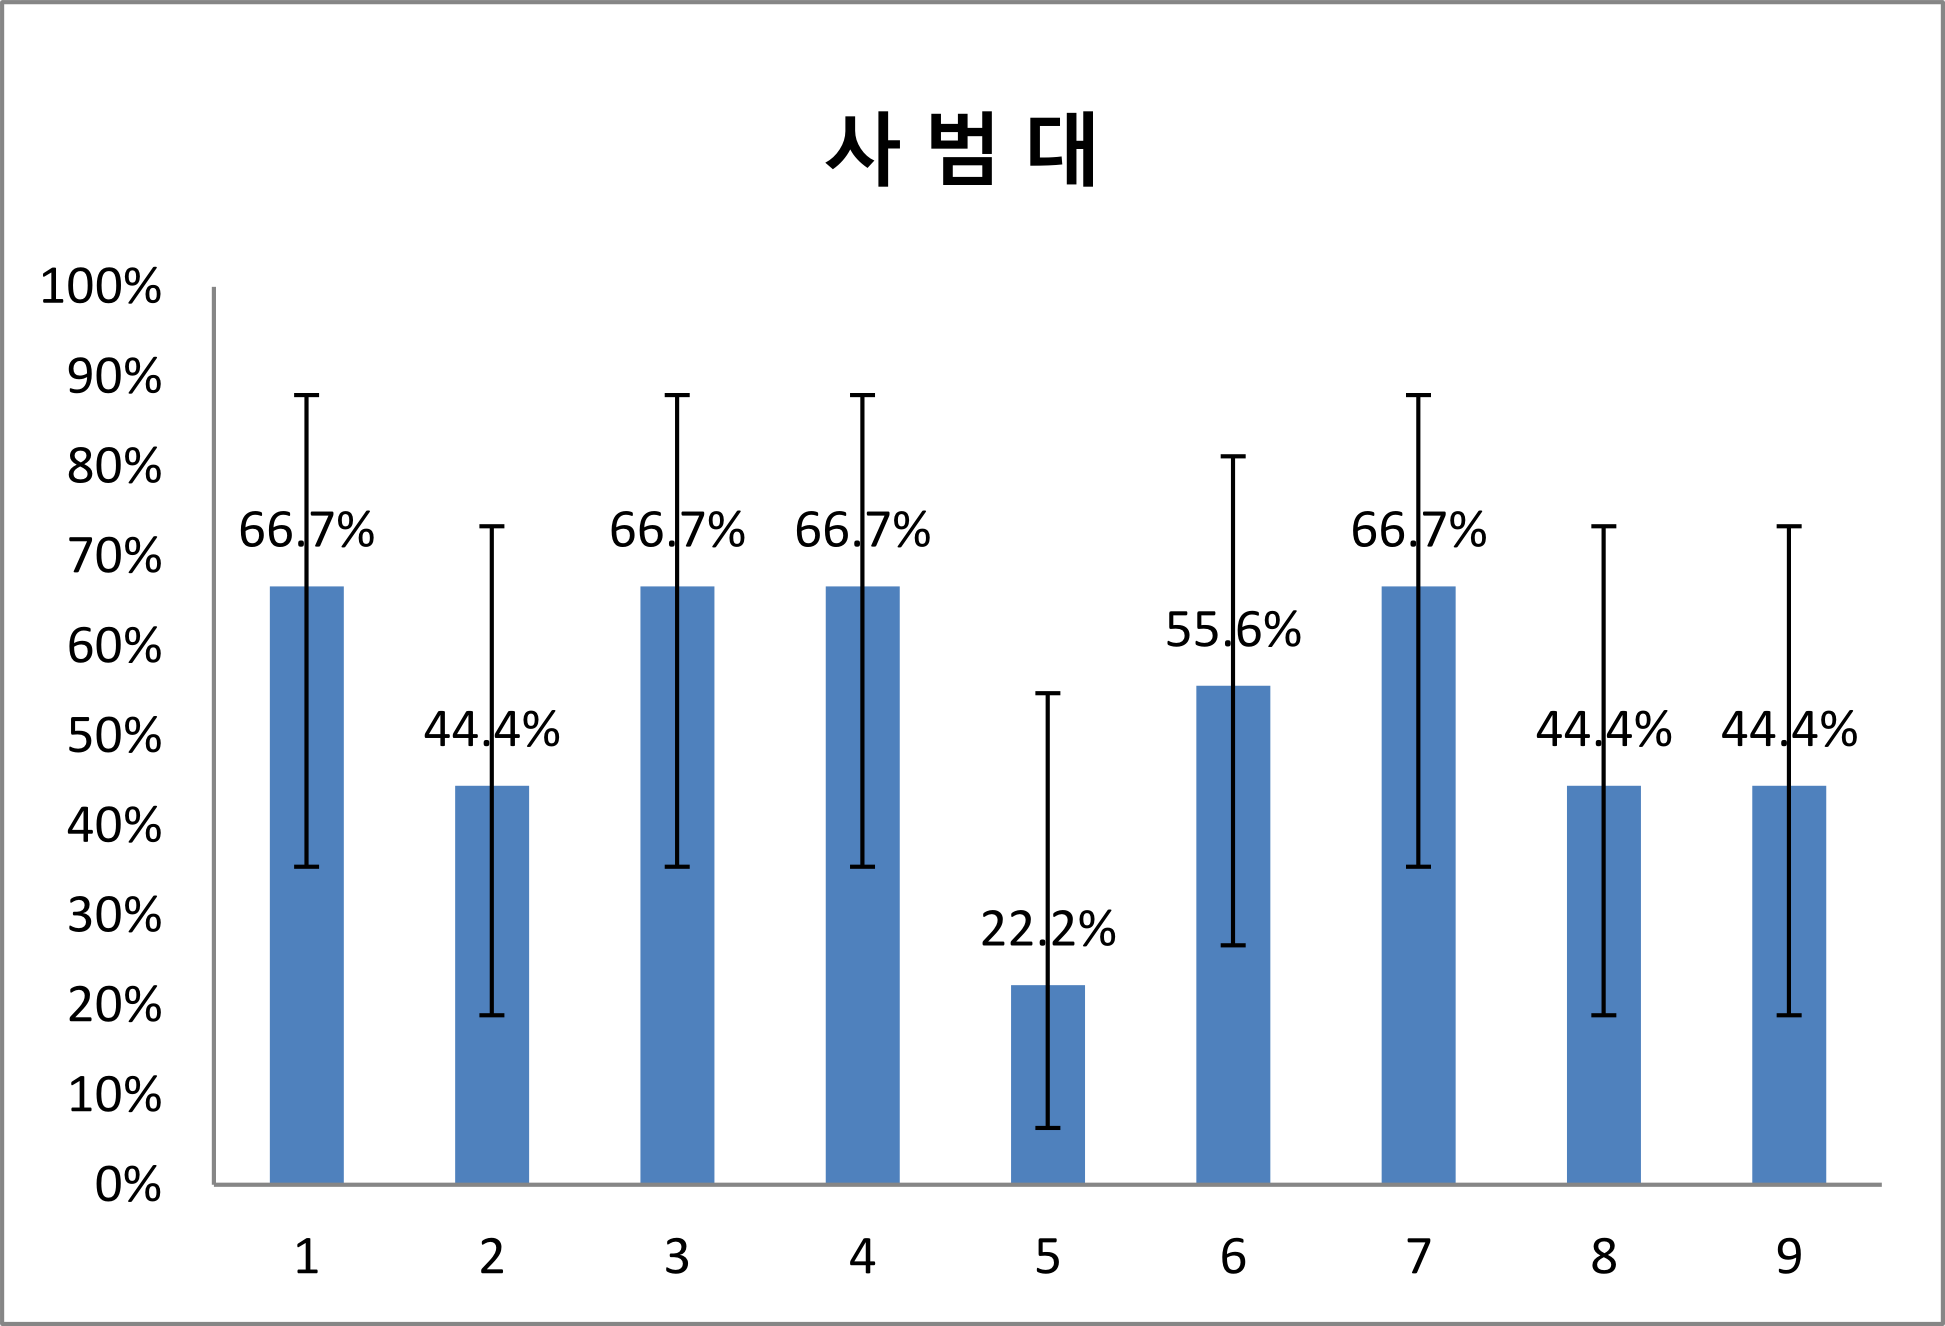
\includegraphics[width=0.45\textwidth]{4_1_3_2}
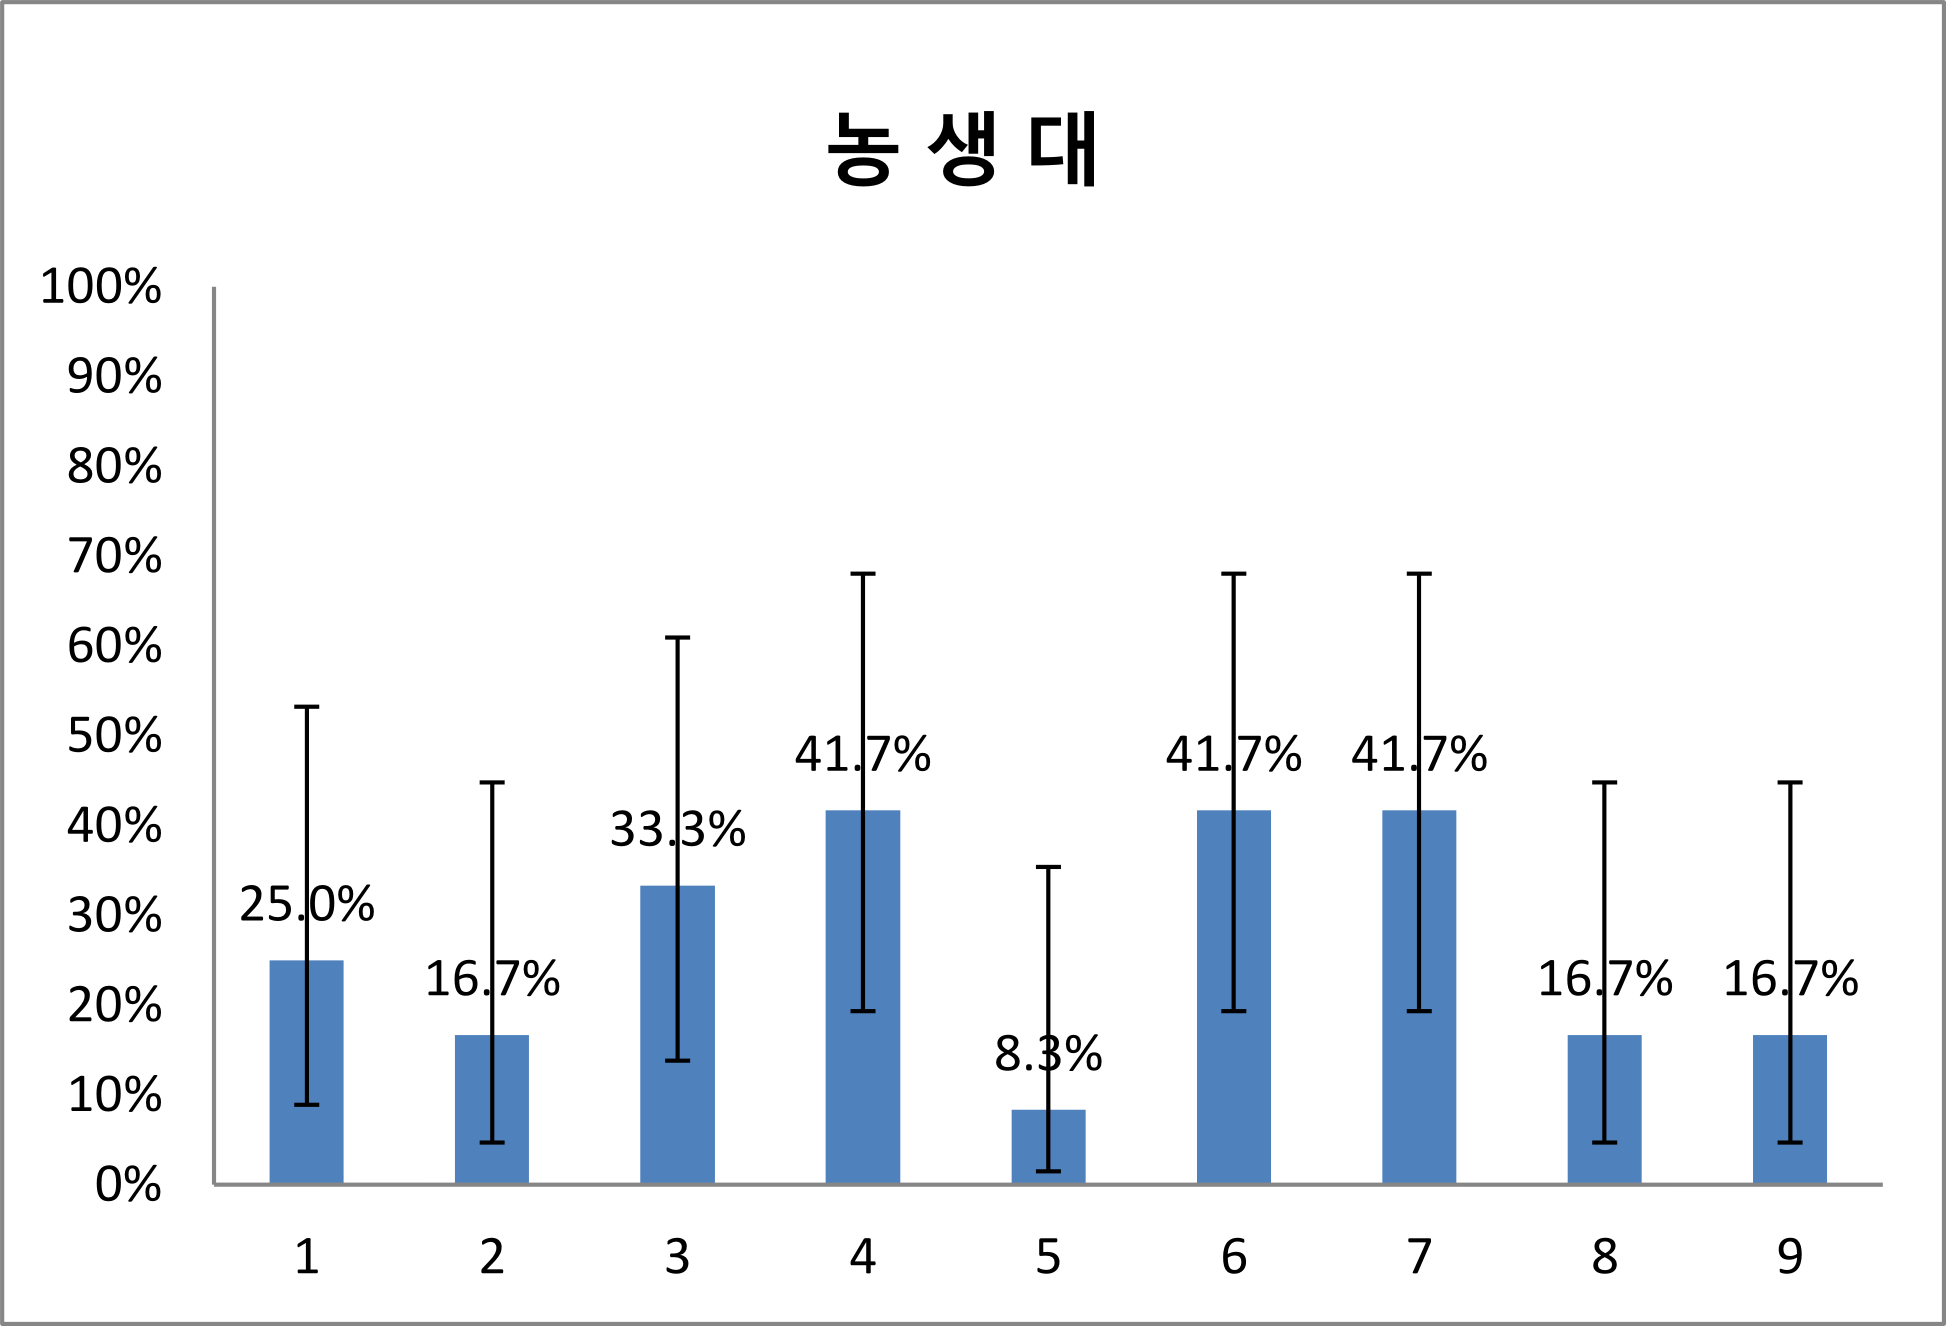
\includegraphics[width=0.45\textwidth]{4_1_3_3}
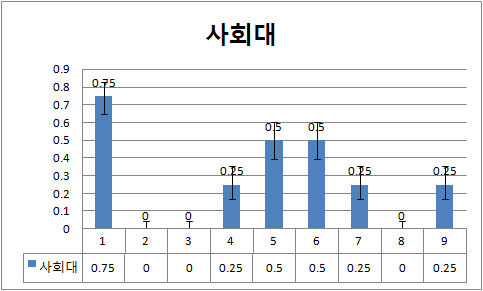
\includegraphics[width=0.45\textwidth]{4_1_3_4}
\centering
\end{figure}

\subsubsection{특정 문제점들에 대한 이용자들의 인식 분석}
설문조사에서 나타난 불편함의 경험률이 실제 이용자들의 불편함을 느끼는 정도에
미치는 영향에 비례하지 않을 수 있다. 따라서 특정 문제점들에 대한 이용자들의
중요성 인식을 설문 조사했다. 설문조사에 따르면 이용자들이 가장 중요한 문제라고
인식하는 문항은 2번으로, 예약자가 예약한 시간에 기다림 없이 바로 강의실을
사용할 수 있어야 한다는 것이다. 문항 점수의 평균은 4.43점으로 문항의 만점이
5점인 것을 고려하면 이용자 대부분이 예약한 시간에 강의실을 이용할 수 있어야
한다고 생각한다는 것을 알 수 있다. 또, 위에서 지적되었던 예약한 강의실에 갔을
때 강의실이 잠겨있어 강의실을 바로 사용하지 못했던 경험이 매우 좋지 못한
경험이라는 것을 알 수 있으며 이 문제를 해결하는 것을 중요하게 고려해야 한다.

그 외에도 예약자가 늦게 왔을 때에도 일행이 강의실에 들어갈 수 있어야 한다는 3번
문항도 3.71점으로 이용자들이 중요한 문제로 인식하고 있다는 것을 알 수 있다.
반면에 예약자가 찾아올 시간에 수위가 자리를 지키는 것에 대한 중요성인 1번
문항의 점수 평균은 3.36점으로 상대적으로 덜 중요하다고 인식한다는 것을 알 수
있다.
\begin{figure}[H]
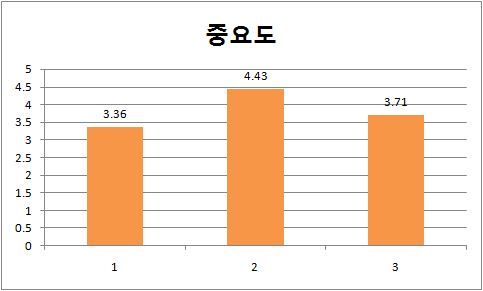
\includegraphics[width=0.8\textwidth]{4_1_4}
\centering
\end{figure}


\subsection{문제의 해결 : 모델 설명}

\subsubsection{강한 블랙 리스트 모델}
위에서 언급한 대로 블랙 리스트 모델은 일반적인 접근을 허용하고, 특정한 대상만을
걸러내기 위하여 CCTV와 이미지 프로세싱 기술을 사용할 것이다. 이 모델은 허용되지
않은 사용자를 이미지 프로세싱을 이용해 걸러내기 때문에 기존의 잠금장치가
존재하지 않는다. 따라서 강한 블랙 리스트 모델은 다음과 같은 특성을 가진다.

\begin{itemize}
\item 모든 강의실의 문은 언제나 열려있다.
\item 강의실은 해당 강의실이 예약된 시간이 아니면 누구도 이용할 수 없다.
\item 강의실은 해당 강의실이 예약된 시간에는 누구라도 이용할 수 있다.
\item 어떤 사용자든 파손 행위 등을 하면 바로 신고된다.
\end{itemize}

\subsubsection{약한 블랙 리스트 모델}
위에서 설명한 강한 블랙 리스트 모델은 이미지 프로세싱이 파손 행위 등을 완벽하게
잡아낼 수 있어 잠금장치가 필요하지 않는다는 가정하에 세워진 모델이다.
잠금장치가 존재하지 않는다는 특성은 모델의 특성을 간략화하는 장점이 있지만,
현재의 이미지 프로세싱은 그렇게 완벽하게 작동하지는 않는다. 또한, 강의실의
특성상 사용자가 사용 중에는 문을 잠글 수 있다.

따라서 잠금장치가 존재하는 새로운 모델을 제시할 것이다. 이 모델을 약한 블랙
리스트 모델이라고 부르도록 하겠다. 약한 블랙 리스트 모델은 다음의 특성을
가진다.
\begin{itemize}
\item 예약자만이 수위의 허가를 받을 수 있다.
\item 잠겨있는 강의실은 수위의 허가를 통해 들어갈 수 있다.
\item 잠겨있지 않은 강의실은 누구나 들어갈 수 있다.
\item 예약된 시간에 문이 열려 있는 강의실은 누구나 이용할 수 있다.
\end{itemize}

\subsubsection{강한 화이트 리스트 모델}
화이트 리스트 모델에서 문은 항상 잠겨있다. 강의실을 사용할 권한이 있는
사람에게만 비밀번호를 알려주어 문을 열 수 있게 해준다. 따라서 강한 화이트
리스트 모델은 다음과 같은 특성을 가진다.
\begin{itemize}
\item 모든 강의실은 잠겨있다.
\item 예약한 사람은 다른 사람의 강의실 출입을 허가할 수 있다.
\item 강의실 문은 허가된 사람만 열 수 있다.
\item 강의실에 들어갈 수 있으면 강의실을 사용할 수 있다.
\end{itemize}

\subsubsection{약한 화이트 리스트 모델}
강한 화이트 리스트 모델에는 한가지 결점이 있다. 강한 화이트 리스트 모델은 모든
강의실이 잠겨있다. 하지만 강의실을 사용 중인 사람이 문을 열어둘 수도 있고,
강의실의 문을 열어두고 강의실을 떠날 수 있기 때문에, 현실적으로 이는 참이
아니다. 약한 화이트 리스트 모델에서는 이를 반영하여 강의실의 문이 잠겨있지 않는
경우를 고려할 것이다. 약한 화이트 리스트 모델이 가지는 특성은 다음과 같다.
\begin{itemize}
\item 예약한 사람은 다른 사람의 강의실 출입을 허가할 수 있다.
\item 강의실 문은 허가된 사람만 열 수 있다.
\item 강의실의 문이 열려 있으면, 누구나 강의실에 들어갈 수 있다.
\item 강의실에 들어갈 수 있으면 누구나 파손 행위 등을 할 수 있다.
\end{itemize}

\subsection{문제 해결책 검증}

\subsubsection{상황 설정}
문제를 쉽게 이해할 수 있기 위해 간단한 상황을 상정하였다. 이 상정된 상황은
일반적으로 확장해도 적용할 수 있다.

예약은 하루에 하나의 시간대만 보겠다고 가정하였다. 또한, 예약할 수 있는
강의실은 301호부터 305호까지이다. 등장하는 인물은 규민, 슬기, 재성, 재찬,
찬민의 다섯 명이며, 예약 상황은 다음과 같다.

\begin{itemize}
\item 재찬은 토요일에 301호를 이용하기로 예약하였다.
\item 재찬은 일요일에 302호를 이용하기로 예약하였다.
\item 슬기는 토요일에 302호를 이용하기로 예약하였다.
\item 슬기는 일요일에 302호를 이용하기로 예약하였다.
\item 슬기는 월요일에 301호를 이용하기로 예약하였다.
\item 슬기는 화요일에 301호를 이용하기로 예약하였다.
\item 수위는 토요일에 자리를 비웠다.
\item 슬기는 일요일에 학교에 오지 않았다.
\item 슬기는 화요일에 학교에 오지 않았다.
\item 재찬은 규민을 토요일 301호 예약에 초대했다.
\item 슬기는 재찬을 토요일 302호 예약에 초대했다.
\item 슬기는 규민을 일요일 302호 예약에 초대했다.
\end{itemize}

\subsubsection{질의 목록}
\begin{enumerate}
\item 예약자가 강의실 이용에 실패하는 경우가 있는가?
\item 허가되지 않은 사용자가 강의실을 이용할 수 있는가?
\item 강의실 물품 파손 행위 등을 할 수 있는가? (이때, 예약한 사람 및 허가된 사용자는 물품 파손 등을 하지 않는다고 가정한다)
\item 수위가 없고, 휴일일 때 강의실을 이용할 수 있는가?
\item 전원이 자리를 비웠을 때 그 사이 강의실 물품 파손 행위 등이 일어날 수 있는가?
\item 허가된 사용자가 강의실을 이용할 수 없는 경우가 있는가?
\end{enumerate}

\subsubsection{기존 모델}

\paragraph{특성}
\begin{itemize}
\item 주말에는 강의실 문이 잠겨 있고, 평일에는 열려 있다.
\item 강의실이 열려있지 않고, 수위가 없으면 누구도 방에 들어갈 수 없다.
\item 방이 열려있지 않고, 수위가 있고 예약자가 없으면, 허가된 사용자는 강의실에 들어갈 수 없다.
\item 문이 열려있지 않고, 수위가 있으면 예약자는 강의실로 들어갈 수 있다.
\end{itemize}

\paragraph{질의 결과}
\begin{enumerate}
\item 재찬이 토요일에 301호를, 슬기가 토요일에 302호 예약을 했지만 이용할 수 없다. 이는 수위가 자리를 비운 상태이기 때문이다.
\item 모든 사람이 모든 강의실에 대해, 평일에는 이용할 수 있다. 이는 평일에 모든 강의실 문이 열려 있기 때문이다.
\item 모든 강의실이 평일에 대해 물품 파손 등의 피해를 볼 수 있다. 이유는 위와 같다.
\item 수위가 없고 휴일일 경우에는, 휴일에 문이 잠겨 있고 문을 열어줄 수위가 없으므로 강의실을 이용할 수 있는 경우가 없다.
\item 월요일에 301호를 예약한 슬기는 자리를 비운 사이 자신의 물건을 도난당할 가능성이 있다. 평일에는 문을 잠그지 않기 때문이다. 화요일에는 슬기가 예약했지만, 예약한 사람이 아무도 오지 않았으므로 강의실 물품 파손 피해를 볼 수 있다.
\item 재찬은 토요일 302호 예약에 초대되었고 규민은 토요일 301호 예약과 일요일 302호 예약에 초대되었지만, 이용할 수 없다. 토요일 예약은 수위가 자리를 비웠기 때문에 이용할 수 없으며, 일요일에는 예약자가 오지 않아서 강의실을 이용할 수 없다.
\end{enumerate}

\subsubsection{강한 블랙 리스트 모델}

\paragraph{특성}
\begin{itemize}
\item 어떤 강의실이 예약되지 않은 시간에는 누구도 그 강의실을 점유할 수 없다.
\item 어떤 강의실이 예약된 시간에 강의실에 들어갈 수 있는 사람들 중 가장 강하게 주장하는 사람이 점유할 수 있다.
\item 허가된 사용자는 가장 우선 순위가 높다.
\item 나머지의 순서는 임의로 정해진다.
\item 강의실이 예약되어있는 시간이지만, 허가된 사용자가 아닌 사람이 점유하고 있으면 파손 피해가 있을 수 있다.
\end{itemize}

\paragraph{질의 결과}
\begin{enumerate}
\item 예약자가 강의실을 이용할 수 없는 경우는 없다. 예약된 시간에는 항상 들어갈 수 있고 우선순위가 가장 높은 사람이기 때문이다.
\item 재찬은 화요일에 301호 강의실을 허가받지 않았는데도 불구하고 점유할 수 있다. 예약한 사람인 슬기가 오지 않았기 때문이다.
\item 화요일 301호 강의실은 파손 피해가 발생할 수 있다. 허가 받지 않은 사람인 재찬이 들어갈 수 있기 때문이다.
\item 토요일에 재찬과 규민은 301호를 점유할 수 있고, 토요일에 재찬과 슬기는 302호를 점유할 수 있다.
\item 예약한 시간에도 파손 피해 등의 문제가 생길 수 있다. 화요일 슬기가 301호를 예약했지만 오지 않았으므로 허가받지 않은 재찬이 들어갈 수 있기 때문이다.
\item 없다. 허가된 사용자는 가장 우선 순위가 높기 때문에 언제든 들어가서 강의실을 점유할 수 있다.
\end{enumerate}

\paragraph{기존 모델과의 차이점}
\hfill\break
기존 모델에선 예약자가 수위를 통해 문을 열어야 강의실을 이용할 수 있었다.
따라서 예약자가 오지 않는다면 허가된 사용자 역시 강의실을 이용할 수 없었다.
하지만 강한 블랙 리스트 모델에서는 애초에 모든 강의실 문이 열려 있으므로
예약자가 설령 오지 않는다 해도 강의실 이용이 가능하다.
그러나 이 모델은 이미지 프로세싱의 기술의 발달이 선행되어야 이용할 수 있는 모델로, 현재 활용할 수는 없다.

\subsubsection{약한 블랙 리스트 모델}

\paragraph{특성}
\begin{itemize}
\item 문은 기본적으로 열어 놓는다.
\item 문이 열려 있으면 누구나 들어가서 문을 잠글 수 있다.
\item 잠긴 문을 열 수 있는 것은 수위 뿐이다.
\end{itemize}

\paragraph{결과}
\begin{enumerate}
\item 수위가 자리를 비웠을 때 예약한 재찬과 슬기는 강의실을 사용할 수 없다. 다른 누군가가 먼저 들어가서 잠갔지만 잠긴 문을 열 수 있는 수위가 없기 때문이다.
\item 찬민은 열려 있던 강의실에 누구보다 빨리 들어간 경우 강의실을 이용할 수 있다. 허가되지 않은 사용자도, 다른 사람보다 먼저 들어가기만 하면 강의실을 이용할 수 있다.
\item 모든 강의실이 평일에 대해 물품 파손 등의 피해를 볼 수 있다. 이유는 위와 같다.
\item 재찬과 슬기는 강의실을 예약했지만 쓸 수 없다. 수위가 없는 경우에는 아무나 먼저 들어가서 잠근 문을 열어줄 수위가 없으므로 강의실을 이용할 수 없다.
\item 재찬과 슬기가 강의실을 잠깐 비운 사이 허가되지 않은 사람 아무나 들어와서 강의실 물품 파손 등의 피해를 입힐 수 있다.
\item 강의실을 모두 재찬은 토요일 302호 예약에 초대되었고 규민은 토요일 301호 예약과 일요일 302호 예약에 초대되었지만, 이용할 수 없다. 토요일 예약은 수위가 자리를 비웠기 때문에 누군가 들어가서 잠근 경우 이용할 수 없으며, 일요일에는 예약자가 오지 않아서 강의실을 이용할 수 없다.
\end{enumerate}

\paragraph{기존 모델과의 차이점}
\hfill\break
이 모델은 기존 모델과 차이가 거의 없다. 다른 점은 휴일에도 기본적으로 문이 열려
있다는 것인데, 만약 누군가 강의실을 선점해서 문을 잠글 경우, 원래 예약했던
사람은 강의실을 이용할 수 없다. 이 문제를 해결하기 위해서 결국 수위의 도움이
필요하므로, 기존 모델과 별로 차이가 없는 모델이라고 할 수 있다.

\subsubsection{약한 화이트 리스트 모델}

\paragraph{추가 가정}
약한 화이트 리스트 모델에서는 강의실 문이 잠겨 있을 수도 있고, 열려 있을 수도 있다. 여기서는 토요일에 302호가 특별히 열려 있다고 가정한다.

\paragraph{질의 결과}
\begin{enumerate}
\item 예약자가 강의실을 이용할 수 없는 경우는 없다. 수위가 있든 없든 이용할 수 있고, 강의실이 잠겨 있어도 일회용 비밀번호를 발급받을 수 있어서 문을 열 수 있기 때문이다.
\item 규민과 재성, 찬민은 예약을 한 적이 없지만, 토요일에 302호를 이용할 수 있다. 토요일 302호는 항상 열려 있기 때문이다.
\item 토요일의 302호는 열려 있기 때문에, 항상 기물 파손의 위협이 존재한다.
\item 수위가 없고 휴일일 때라도 예약자 및 허가된 사용자는 자신에게 허가된 강의실을 이용할 수 있다. 일회용 비밀번호는 예약자가 허가된 사용자에게 공유할 수 있고, 허가된 사용자는 받은 일회용 비밀번호를 이용하여 강의실 문을 열 수 있기 때문이다.
\item 토요일에 302호를 예약한 슬기는 강의실을 비웠을 때 자신의 물품을 도난당할 가능성이 있다. 이는 토요일에 302호가 문이 열려 있기 때문이다.
\item 허가된 사용자가 예약된 강의실을 이용할 수 없는 경우는 없다. 이는 위에 언급된 이유와 같다.
\end{enumerate}

\paragraph{기존 모델과의 차이점}
\hfill\break
기존 모델에서는 수위라는 존재가 있어야 문을 열 수 있었고, 따라서 휴일에 예약한
경우 수위가 없으면 문을 열 수 없었다. 그러나 약한 화이트 리스트 모델에서는 이
사항이 개선되어, 수위의 유무와 관계없이 강의실을 이용할 수 있다.
또한, 기존 모델에서는 예약자가 부득이한 사정으로 오지 못하게 되었을 때, 허가된
사용자라도 강의실을 이용할 수 없는 불편함이 있었다. 그러나 약한 화이트 리스트
모델에서는 예약자가 오지 못한다고 하더라도 허가된 사용자에게 일회용 비밀번호를
쉽게 보낼 수 있기 때문에 허가된 사용자가 강의실을 이용하는 데 불편이 없다.

\section{결론}

\subsection{요약과 함의}
강의실 예약 시스템은 학내 동아리 활동, 학술 모임 등을 위해 쓰이는 유용한
시스템이며, 설문조사 결과에서도 나타났듯이 약 40\%의 학생이 이용하는
시스템이다. 그러나 현행 강의실 예약 시스템은 예약 자체는 전산화가 완료되어
인터넷으로 간편하게 예약할 수 있지만, 실제로 예약한 시간에 강의실을 이용하기
위해서는 수위라는 제삼자를 통한 인증이 필요하다.

제시한 화이트 리스트 모델을 통해 강의실 예약 시스템의 완전한 자동화를 이룰 수
있으며, 이는 학내 구성원들이 강의실 예약 시스템을 이용할 때 기존 시스템보다 더
편리하게 이용할 수 있음을 의미한다. 화이트 리스트 모델을 적용할 경우 예약한
시간에 수위가 자리를 비웠을 경우 기다리는 시간을 없애고, 예약자가 늦게 도착했을
때 함께 강의실을 이용할 사람이 예약자를 기다리는 일 없이 강의실을 바로 이용할
수 있게 된다.

그러나 약한 블랙 리스트 모델의 경우, 기존의 결과와 큰 차이가 나지 않으며,
휴일에 문을 잠그지 않는 시스템은 오히려 보안 면에서 기존 모델보다 취약한 모습을
보였다. 따라서 약한 블랙 리스트 모델은 기존의 모델을 대체하기 힘들다.

강한 블랙 리스트는 잠금 장치가 없어도 이미지 프로세싱을 통해 예약 시간 외의
시간에 사람이 강의실에 있어 움직임을 보이면 수위에게 바로 알림이 가는
시스템으로, 약한 블랙 리스트 모델이 가지고 있던 단점을 극복하고 기존 모델을
대신해 쓸 수 있을 것이다. 다만 강한 블랙 리스트 모델을 도입하기 위한 이미지
프로세싱 기술이 아직 그 수준에 이르지 못했고, 기술의 발달로 도입할 수 있게
된다면 이 역시 고려하면 좋을 것이다.

이 연구 결과는 기존 예약 시스템을 개선하거나 새 예약 시스템을 도입할 때 참고할
만한 모델이 될 수 있을 것이다.

\subsection{연구의 한계}
이 연구에서는 기존 시스템을 제시한 화이트 리스트, 블랙 리스트 모델로 교체하였을
때 생기는 이득만을 고려했을 뿐, 예약 시스템을 변경했을 때 생기는 비용 문제는
고려하지 않았다.
화이트 리스트의 경우, 해당 시스템을 구축하기 위해서는 현재 강의실을 잠그는 데
이용되는 자물쇠를 OTP 자물쇠로 교체하는데 비용이 발생하고, OTP 비밀번호를
예약자에게 전송할 수 있어야 하므로 이 시스템을 구축하는 비용이 추가로 발생한다.
블랙 리스트의 경우, 현재 CCTV가 강의실 대부분에 있으나, 소형 강의실에는 아직
CCTV가 없는 곳도 존재한다. 그러므로 이런 강의실에 CCTV를 설치하는 비용이 발생할
수 있다.
하지만 보안상의 이유로 CCTV는 점점 보급되어 가고 있고, 교실의 출입문도 노후화로
개선 작업이 필요하므로 이런 비용을 고려하더라도 이번 연구가 의미 없는 것은
아니다.

\subsection{새로운 연구 제안}
본 연구는 예약 자체를 다루지는 않고, 예약한 이후 강의실 이용에 관한 개선
방안만을 제시하였다. 새로운 연구에서는 예약 자체에 대한 개선안을 포함하고 본
연구의 결과를 참조하여, 현행 강의실 예약 시스템보다 더 편리한 예약 시스템에
대해 연구할 수 있을 것으로 기대한다.
또한, 위에서 언급하였듯이 본 연구는 비용의 문제를 고려하지 않았기 때문에
추가되는 비용과 교체를 통해 얻을 수 있는 이익을 비교하는 것도 좋은 연구가 될
것이다.

\section{참고문헌}
\begin{enumerate}
\item 김지영, 2013, “난수를 이용한 전자식 잠금장치 및 그 제어방법”, 등록특허 10-1228611, 대한민국특허청.
\item Shah, Mubarak, Omar Javed, and Khurram Shafique, 2007, “Automated visual surveillance in realistic scenarios.”, IEEE MultiMedia 14.1.
\item Davies, Antony C., and Sergio A. Velastin, 2005, “Progress in 1computational intelligence to support cctv surveillance systems.”, International Scientific Journal of Computing 4.3.
\end{enumerate}

\section{부록}
\subsection{설문조사지 : 서울대학교 강의실 예약 및 이용 편의성 조사}
귀한 시간 내주셔서 감사합니다. 이 설문은 과학 기술과 글쓰기(031.004) 수업의 논문 작성을 위해 진행되고 있습니다. 논문의 주제는 예약한 강의실을 사용하는 데 있어서 생기는 불편함 해결로, 예약한 강의실을 사용하는데 어떠한 불편함이 있는가를 조사하고 있습니다. (본 설문은 1분 정도 소요됩니다.)
\begin{enumerate}
\item 현재 다니고 있는/마지막으로 다닌 단과대학(주전공)은 무엇입니까?\\
(* 이 질문은 주로 예약하는 강의실 건물의 대략적인 위치를 알아보기 위한 것입니다.)\\
간호대 경영대 공대(아랫공대) 공대(윗공대)\\
농생대 법대 사범대 사회대\\
생활과학대 수의대 약대 음/미대\\
의대 인문대 자연대 자유전공
\item 최근 4년 이내에 강의실 예약 시스템을 이용해 본 적이 있습니까?\\
예\\
아니오 (이 설문지 작성을 중지하세요.)
\item 아래 질문들에 대해 예/아니오로 선택해주세요.
\begin{center}
\begin{tabular}{ | l | c | c | }
\hline
질문 & 예 & 아니오 \\
\hline
예약 후 확인을 위해 수위에게 예약 신청서를 요구 받은 적이 있습니까? & & \\
\hline
수위가 예약 시스템의 존재를 몰라 불편을 겪었던 적이 있습니까? & & \\
\hline
예약 후 수위가 자리를 비워 불편을 겪은 적이 있습니까? & & \\
\hline
예약 후 강의실에 갔더니 문이 잠겨 있어 불편을 겪은 적이 있습니까? & & \\
\hline
예약하지 않은 사람이 예약한 강의실을 선점하여 불편을 겪은 적이 있습니까? & & \\
\hline
예약 시간 연장의 필요성을 느낀 적이 있습니까? & & \\
\hline
이미 예약한 시간을 변경하거나, 예약을 취소해야 했던 적이 있습니까? & & \\
\hline
강의실 사용 중 (식사 등의 이유로) 전원이 자리를 비웠던 적이 있습니까? & & \\
\hline
예약자가 늦게 도착하거나 불참하게 되어 불편을 겪은 적이 있습니까? & & \\
\hline
\end{tabular}
\end{center}
\item 아래 질문들에 대해 1점(전혀 중요하지 않다)에서 5점(아주 중요하다)으로 점수를 매겨주세요.
\begin{center}
\begin{tabular}{ | p{12cm} | c | c | c | c | c | }
\hline
질문 & 1 & 2 & 3 & 4 & 5 \\
\hline
예약자가 찾아올 시간에 수위가 자리를 지키고 있는 것이 얼마나 중요하다고 생각하십니까? & & & & & \\
\hline
예약자가 예약한 시간에 기다림 없이 바로 강의실을 사용할 수 있는 것이 얼마나 중요하다고 생각하십니까? & & & & & \\
\hline
예약자가 늦게 왔을 때에도 일행이 강의실에 들어갈 수 있게 하는 것이 얼마나 중요하다고 생각하십니까? & & & & & \\
\hline
\end{tabular}
\end{center}
\end{enumerate}
\end{document}
